
\documentclass[a4paper]{article}
\usepackage[pdftex]{graphicx}
\usepackage[utf8]{inputenc}
\usepackage{enumerate}
\usepackage{siunitx}
\sisetup{locale=DE} 
\usepackage{icomma}
\usepackage{amssymb}
\usepackage{tikz}
\usepackage{href-ul}
\hypersetup{
	colorlinks=true,
	linkcolor=blue,
	urlcolor=blue}
\usepackage{geometry}
\geometry{a4paper, top=15mm, left=15mm, right=15mm, bottom=15mm,
	headsep=10mm, footskip=12mm}

\begin{document}
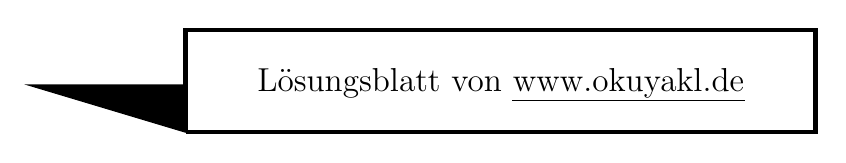
\begin{tikzpicture}(10,3)
	\draw[ultra thick](2,0) --(10,0) -- (10,1.3) --(2,1.3) -- (2,0);
	\draw[fill=black](2,0)-- (0,.6) -- (2,.6) -- (2,0);
	\node at (6,.6) {\large Lösungsblatt von \href{https://www.okuyakl.de}{www.okuyakl.de}};
\end{tikzpicture}
\vspace{0.5 cm}

\noindent{\bf Aufgabe 1.}\\
\begin{minipage}{0.65\textwidth}
    Der Gesamtwiderstand setzt sich zusammen aus dem ohmschen Widerstand des Kondensators $R$ auf der reellen Achse und dem Blindwiderstand des Kondensators $X=-{ 1 \over \omega C}$ auf der imaginären Achse. Der Betrag des komplexen Gesamtwiderstands $Z$ ist nach dem Satz des Pythagoras:
    $$
    \begin{array}{rcll}
    Z^2 & = & R^2 + \left( { 1 \over \omega C} \right)^2\\
    Z^2 & = & R^2 + \left( { 1 \over 2\pi f \cdot C} \right)^2\\
    Z & = & \sqrt{R^2 + \left( { 1 \over 4\pi^2 f^2 \cdot C^2} \right)}
    \end{array}
    $$
\end{minipage}
\begin{minipage}{0.35\textwidth}
\includegraphics[width=6 cm]{zeidi234.pdf}
\end{minipage}
\vspace{0.5 cm}

\noindent{\bf Aufgabe 2. a)}\\
Wenn am ohmschen Widerstand die Spannung $U_{R,1}$ abfällt, dann fließt durch ihn ein Strom der Stärke:
$$ I = {U \over R} = {\SI{11,2}{\volt} \over \SI{40e3}{\ohm}} = \SI{0,28}{\milli\ampere}$$
Die Effektivspannung, die am Kondensator abfällt, ist nach dem Zeigerdiagramm:
$$
\begin{array}{rcll}
U_{C,1}^2 & = & U_{eff}^2 - U_{R,1}^2 \\
U_{C,1} & = & \sqrt{U_{eff}^2 - U_{R,1}^2 }\\
U_{C,1} & = & \sqrt{(\SI{12}{\volt})^2 - (\SI{11,2}{\volt})^2} = \SI{4,3}{\volt}
\end{array}
$$
Daraus errechnet sich ein Blindwiderstand von 
$$X = {\SI{4,3}{\volt} \over \SI{0,28}{\milli\ampere}}= \SI{15,4}{\kilo\ohm} $$
Wir setzen gleich mit  $X={ 1 \over \omega C}$ und lösen nach $C$ auf:
$$C = {1 \over 2\pi f X} = {{1 \over 2\pi \cdot \SI{520}{\hertz} \cdot \SI{15,4e3}{\ohm}}} = \SI{20e-9}{\farad} = \SI{20}{\nano\farad}$$
Einheitencheck:
$$\SI{}{1 \over {\second^{-1}\cdot \volt \cdot \ampere^{-1}}}= \SI{}{\ampere\second \over \volt} = F $$
Für die Phasenverschiebung $\varphi_1$ zwischen Stromstärke und Eingangsspannung gilt:
$$\tan\varphi_1= {X \over R} \quad \Rightarrow \quad \varphi_1 = \arctan\left({X \over R} \right)= \arctan \left({\SI{15,4}{\kilo\ohm} \over \SI{40}{\kilo\ohm}} \right) = 21^\circ$$
\vspace{0.5 cm}

\noindent{\bf Aufgabe 2. b)}\\
Die Wirkleistung $P_1$ ist die Leistung, die am ohmschen Widerstand in Joulesche Wärme umgewandelt wird:
$$P_1 = {U_{R,eff,1}^2 \over R} = {(\SI{11,2}{\volt})^2 \over \SI{40e3}{\ohm}} = \SI{3,1}{\milli\watt}$$
\vspace{0.5 cm}

\noindent{\bf Aufgabe 3. a)}\\
Die Stromstärke $I_eff$ ist, da es sich um eine Reihenschaltung handelt, nach dem Kirchhoffschen Gesetz im gesamten Stromkreis gleich; also ist die frequenzabhängige Effektivstromstärke $I_{R,eff}(f)$ gleich der effektiven Gesamtstromstärke  $I_{eff}$: 
$$
\renewcommand{\arraystretch}{2}
\begin{array}{rcll}
 I_{R,eff}(f) & = & I_{eff}  \\
 {U_{R,eff}(f) \over R} & = & {U_{eff}\over Z} &|\cdot R\\
 U_{R,eff}(f) & = & {R \over Z} \cdot U_{eff} \\
 U_{R,eff}(f) & = & {R \over \sqrt{R^2 + {1 \over 4 \pi^2 C^2} \cdot {1 \over f^2}}} \cdot U_{eff}
\end{array}
$$ 
\vspace{0.5 cm}

\noindent{\bf Aufgabe 3. b)}\\
Wenn die Effektivwerte der Spannungen am Kondensator und am ohmschen Widerstand gleich groß sind, folgern wir für die Grenzfrequenz:
$$ 
\renewcommand{\arraystretch}{2}
\begin{array}{rcll}
\varphi & = & 45^\circ \Rightarrow & X = R \\
     R  & = & {1 \over 2 \pi f \cdot C}  & | \cdot f \quad :R\\
     f_g  & = & {1 \over 2 \pi R \cdot C}\\
     f_g  & = & {1 \over 2 \pi \cdot \SI{40e3}{\ohm} \cdot \SI{20e-9}{\farad}}\\
     f_g  & = & \SI{200}{\hertz} 
\end{array}
$$ 
Einheitencheck:
$$\SI{}{1 \over \volt\cdot \ampere^{-1}\cdot \ampere\cdot \second \cdot \volt^{-1}}= \SI{}{\second^{-1}}=\SI{}{\hertz}$$
Die Effektivwerte der Spannungen $U_{R,eff}$ und $U_{C_eff}$ sind gleich; vektoriell addiert ergeben sie $U_{eff}=\SI{12}{\volt}$. Also ist:
$$
\renewcommand{\arraystretch}{2}
\begin{array}{rcll}
U_{eff}^2 & = & U_{R,eff}^2+ U_{C_eff}^2 & | U_{R,eff} = U_{C_eff}\\
U_{eff}^2 & = & 2\cdot U_{R,eff}^2 &| \sqrt{\quad} \\
U_{eff}   & = & \sqrt{2} \cdot U_{R,eff} \\
U_{R,eff} & = & {U_{eff} \over \sqrt{2}} \\
U_{R,eff} & = & {\SI{12}{\volt} \over \sqrt{2}} & = \SI{8,5}{\volt} = U_{C_eff}
\end{array}
$$ 
Beide Effektivwerte haben den Wert $\SI{8,5}{\volt}$.
\vspace{0.5 cm}

\noindent{\bf Aufgabe 3. c)}\\
Wenn die Frequenz $f$ sehr groß wird, dann nähert sich der zweite Summand
unter der Wurzel Null an und damit wird der Faktor ${R \over Z}\approx 1$ vor $U_{eff}$. Damit werden die beiden Spannungswerte links und rechts praktisch gleich groß. Dies deckt sich auch mit der Tatsache, dass der Kondensator mit steigender Frequenz immer besser leitet, bis schließlich bei sehr hohen Frequenzen sein Widerstand vernachlässigbar klein gegenüber dem vorgeschalteten ohmschen Widerstand wird.  

\begin{center}
	\includegraphics[width=7 cm]{../../viecher/endcomic.pdf}
	
	Hier geht es zurück zum \href{https://www.okuyakl.de/phys/p13wekoL234/aa234.pdf}{Aufgabenblatt}
\end{center}

\end{document}